\documentclass[12pt,english]{article}
\usepackage[utf8]{inputenc}
\usepackage{tgpagella} % Palatino text only
\usepackage{mathpazo}  % Palatino math & text
\usepackage[left=1.5in,right=1.5in,top=1.5in,bottom=1.5in]{geometry}
% \linespread{1.5}
% \usepackage[super,comma,sort]{natbib}
\usepackage[round,sort&compress]{natbib}
\usepackage{url} % [hyphens]
\usepackage[hyperpageref]{backref} % back references biblio. Needs latexmk at compilation.
\usepackage[pagebackref]{hyperref}
% \usepackage{multibib} % incompatible with backref
\hypersetup{
  colorlinks=true, % breaklinks=true,
  urlcolor=purple,    % color of external links
  linkcolor=blue,  % color of toc, list of figs etc.
  citecolor=violet,   % color of links to bibliography
}
\usepackage{bm}
\usepackage{indentfirst}
\usepackage{tocbibind}
\setcitestyle{aysep={}} 
\usepackage{amsmath}
\usepackage{amssymb}
\usepackage{eurosym}
\usepackage{amsfonts}
\usepackage{enumerate}
\usepackage{babel}
\usepackage{caption}
\usepackage{supertabular}
\usepackage{tabularx}
\usepackage{float}
\usepackage{dsfont}
\usepackage{fancyvrb}
\usepackage{verbatim}
\usepackage{enumitem}
\usepackage{setspace}
\usepackage{comment}
\usepackage{subcaption}
\usepackage{graphicx}
\usepackage{tikz}
\usepackage{gensymb}
\usepackage{textcomp}

\usepackage{tabulary}
\usepackage{tabularx}
\usepackage{booktabs}
\usepackage{fullpage}
\usepackage{morefloats}
\usepackage{makecell}
\usepackage{lscape}
\usepackage{pdflscape}
\usepackage{longtable}
\usepackage{rotating}
\usepackage{xcolor}% header
\usepackage{titlesec} % To change size of Bibliography heading
\usepackage{fancyhdr}

% Header on every page except frontpage (handled by tikz)
% \pagestyle{fancy}% header
% \renewcommand{\headrulewidth}{0pt} % removes horizontal line from header
% \setlength{\headheight}{62pt} % adjust the nb of pt here and below if there is a warning
% \addtolength{\topmargin}{-62pt}
% \fancyhead[R]{} % removes section title from header
% \fancyhead[L]{} % removes section title from header
% \chead{\href{http://global-redistribution-advocates.org}{
\includegraphics[height=1cm]{../figures/policies/logo_full_white_bg}}\\ \quad }

\usepackage{tocloft}
\usepackage{titletoc}
\usepackage{csquotes}
\usepackage{tcolorbox}
\usepackage[export]{adjustbox}
\usepackage[anythingbreaks]{breakurl} % for links
\usepackage{multicol}
\newsavebox\ltmcbox % For net gain table over two columns
%\usepackage[nomarkers,figuresonly]{endfloat} % Figures at the end
%\usepackage[section,below]{placeins} % Floats placed in the section they appear in.
\renewcommand{\floatpagefraction}{.9}

\title{Revenues and transfers from global taxes %\\ Technical Note
} 

\author{\textcolor{white}{Adrien Fabre\footnote{\textcolor{black}{The author is Adrien Fabre, CNRS researcher in economics at CIRED. E-mail: adrien.fabre@cnrs.fr.}}}
%\footnote{CNRS researcher in economics at CIRED. E-mail: adrien.fabre@cnrs.fr.}
} 
% \author{Global Redistribution Advocates\footnote{The author is Adrien Fabre, CNRS researcher in economics at CIRED. E-mail: adrien.fabre@cnrs.fr.}} 

% TODO? Ideas from Andreas Bummel. Reduce the endorsement threshold 1M => 500k. Cut the budget (no staffers, 30M per list). Widen the mandate (though not a condition for DwB support): say the assembly would primarily work on climate but could propose things on any domain.

\date{\today{} -- \href{https://github.com/bixiou/global_tax_attitudes/raw/main/paper/policy_brief_taxes.pdf}{Link to most recent version}} 

\begin{document}

\maketitle
\tikz [remember picture, overlay] %
\node [shift={(5.5cm,-1.5cm)}] at (current page.north west) % north west
[anchor=north west] % north west
{\href{http://global-redistribution-advocates.org}{
\includegraphics[height=1.3cm]{../figures/policies/logo_full_white_bg}}};


\section{Summary}\label{sec:intro}

We estimate the tax revenues and their allocation by country, from five global taxes: a tax on wealth above \$100 million, a small carbon tax, % carbon tax is the only one whose transfers are based on GDP
a financial transaction tax, a tax on  maritime fuel and one on aviation fuel. \$1.9 trillion is collected (1.8\% of the world GDP). For most taxes, revenues are returned to each country in proportion to their adult population (except for the wealth tax, which finances poorer countries more). The combination of these taxes and transfers entail \$1 trillion in North--South transfers.
% 850+356+327+223+104 # wealth + carbon + FTT + Aviation + Maritime 
% # Total transfer: 973G (52%)
% 590+94+207+106+53 # 1050 - interactions between taxes

\begin{figure}[h!] 
    \caption{Net tax gain from the combination of new global taxes and transfers, by country.}\label{fig:gain_taxes}
    \makebox[\textwidth][c]{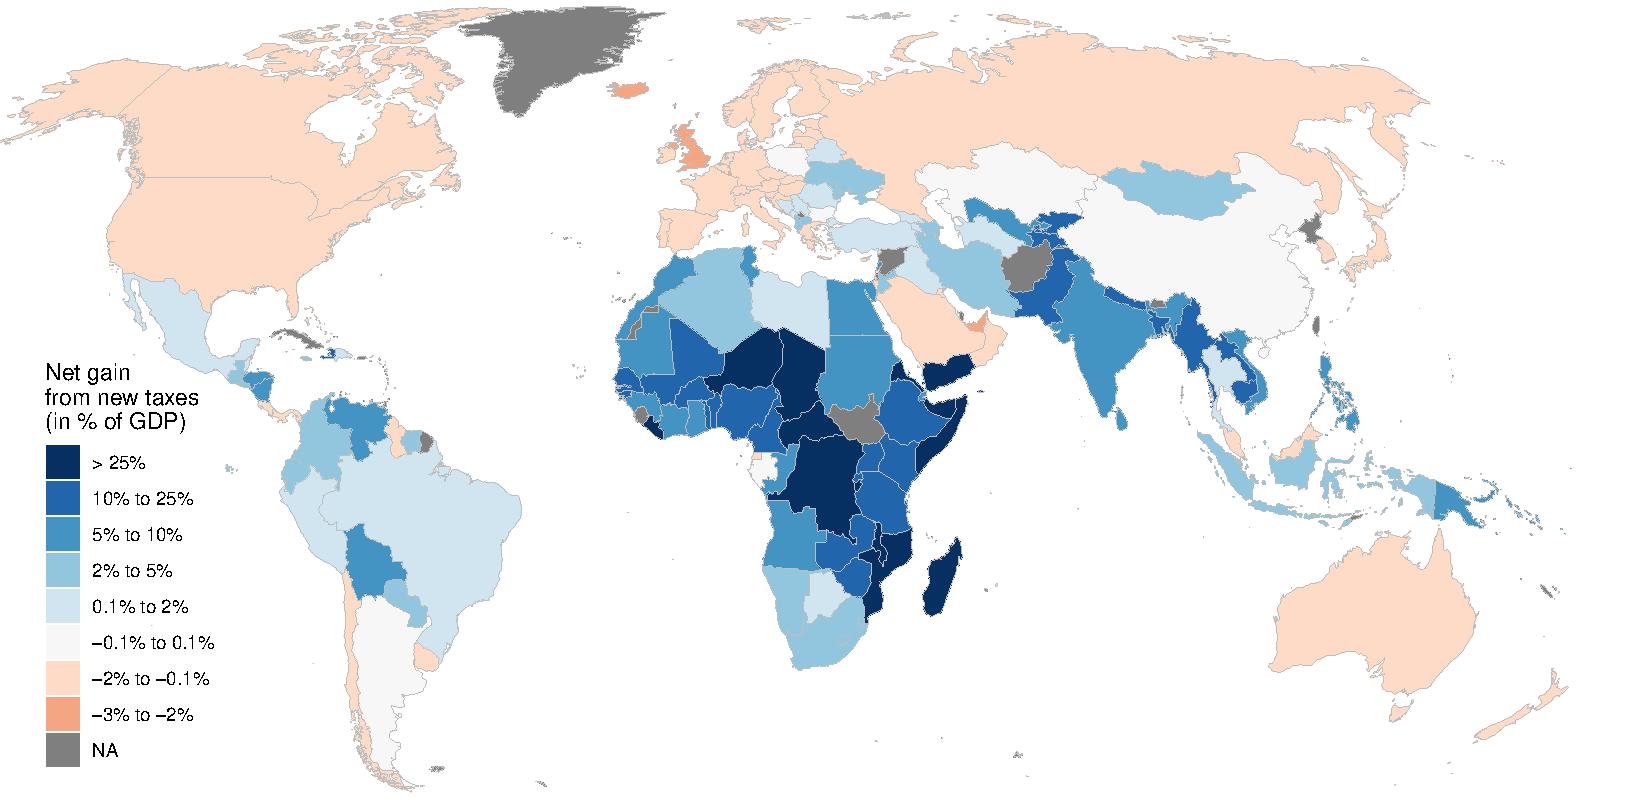
\includegraphics[width=1\textwidth]{../figures/maps/net_gain_over_gdp_all_taxes.pdf}} 
\end{figure}

\clearpage
\begin{table}[!h]
  \caption{\label{tab:revenue_transfers}Net tax gain and revenues collected from global taxes (in \% of GDP).}
  \makebox[\textwidth][c]{
  
\begin{tabular}[t]{lcccccc}
\toprule
  & \makecell{Net gain\\from taxes\\\& transfers} & \makecell{Wealth Tax\\(3\% above\\100M)} & \makecell{Financial\\Transactions\\Tax} & \makecell{Carbon\\Tax\\(10\$/tCO$_\text{2}$)} & \makecell{Maritime\\fuel tax\\(100\$/tCO$_\text{2}$)} & \makecell{Aviation\\fuel tax\\(300\$/tCO$_\text{2}$)}\\
\midrule
World & 0.0 & 0.72 & 0.32 & 0.33 & 0.10 & 0.22\\
Afghanistan & 53.9 & 0.29 & 0.58 & 0.88 & 0.01 & 1.86\\
DRC & 28.4 & 0.32 & 0.13 & 0.10 & 0.11 & 0.10\\
Myanmar & 20.0 & 0.36 & 0.51 & 0.35 & 0.04 & 0.55\\
Sudan & 19.5 & 0.34 & 0.40 & 0.47 & 0.05 & 0.67\\
Uganda & 18.5 & 0.34 & 0.20 & 0.15 & 0.01 & 0.68\\
Ethiopia & 17.7 & 0.35 & 0.14 & 0.12 & 0.00 & 0.45\\
Tanzania & 15.2 & 0.36 & 0.22 & 0.20 & 0.02 & 0.55\\
Pakistan & 13.7 & 0.02 & 0.35 & 0.49 & 0.04 & 0.45\\
Nigeria & 9.0 & 0.10 & 0.24 & 0.34 & 0.35 & 0.35\\
Kenya & 9.0 & 0.39 & 0.15 & 0.18 & 0.02 & 0.32\\
Bangladesh & 8.2 & 0.03 & 0.13 & 0.17 & 0.02 & 0.08\\
India & 8.0 & 1.26 & 0.26 & 0.61 & 0.05 & 0.17\\
Vietnam & 5.4 & 0.01 & 0.17 & 0.50 & 0.11 & 0.16\\
Morocco & 5.0 & 0.44 & 0.23 & 0.49 & 0.18 & 0.46\\
Egypt & 4.5 & 0.44 & 0.29 & 0.63 & 0.07 & 0.20\\
Philippines & 4.3 & 0.28 & 0.19 & 0.22 & 0.03 & 0.37\\
Ukraine & 3.9 & 0.46 & 0.21 & 0.98 & 0.30 & 0.19\\
Indonesia & 3.7 & 0.25 & 0.23 & 0.45 & 0.23 & 0.32\\
Iran & 3.7 & 0.45 & 0.37 & 1.63 & 0.39 & 0.22\\
Algeria & 3.3 & 0.46 & 0.26 & 0.72 & 0.18 & 0.14\\
Colombia & 2.0 & 0.49 & 0.20 & 0.24 & 0.36 & 0.30\\
South Africa & 1.9 & 0.33 & 0.19 & 1.12 & 0.53 & 0.10\\
Thailand & 1.6 & 0.49 & 0.25 & 0.61 & 0.20 & 0.79\\
Iraq & 1.1 & 0.47 & 0.33 & 1.00 & 1.34 & 0.12\\
Brazil & 0.8 & 0.60 & 0.17 & 0.29 & 0.57 & 0.23\\
Turkey & 0.7 & 0.13 & 0.24 & 0.45 & 0.10 & 0.37\\
Mexico & 0.4 & 0.59 & 0.17 & 0.30 & 0.05 & 0.22\\
Argentina & 0.3 & 0.54 & 0.15 & 0.35 & 0.18 & 0.23\\
Poland & 0.2 & 0.11 & 0.16 & 0.44 & 0.07 & 0.10\\
China & 0.0 & 1.06 & 0.10 & 0.58 & 0.05 & 0.15\\
Russia & -0.2 & 0.87 & 0.18 & 0.79 & 0.16 & 0.24\\
Italy & -0.6 & 0.35 & 0.17 & 0.13 & 0.04 & 0.15\\
South Korea & -0.6 & 0.31 & 0.11 & 0.30 & 0.16 & 0.20\\
Japan & -0.7 & 0.22 & 0.40 & 0.23 & 0.05 & 0.14\\
Spain & -0.7 & 0.24 & 0.22 & 0.14 & 0.06 & 0.37\\
Saudi Arabia & -0.8 & 0.11 & 0.15 & 0.59 & 0.52 & 0.25\\
Germany & -0.9 & 0.50 & 0.22 & 0.16 & 0.06 & 0.15\\
Canada & -1.0 & 0.59 & 0.09 & 0.27 & 0.08 & 0.26\\
France & -1.3 & 0.80 & 0.33 & 0.10 & 0.02 & 0.20\\
United States & -1.5 & 0.90 & 0.27 & 0.19 & 0.03 & 0.21\\
United Kingdom & -2.9 & 0.25 & 2.36 & 0.12 & 0.04 & 0.28\\
\bottomrule
\end{tabular} % add \midrule after World
} \end{table}
\clearpage

\section{Tax on ultra-high wealth}\label{sec:wealth}

% Under its G20 presidency, Brazil commissionned a report on a global tax on ultra-high wealth. Indeed, the richest pay less taxes than average people in proportion to their contributive capacity, as most of their income is in the form of unrealized capital gains not subject to taxation. The report by \cite{zucman_blueprint_2024} proposes a top-up tax on the wealth of individual owning more than \$100 million, to collect the missing income tax revenue. With a 3\% top-up tax, a billionaire who already pays taxes amounting to 1\% of its wealth would be liable to an additional 2\% tax. Although a top-up tax may be 

We simulate a 3\% tax on all individual wealth in excess of \$100 million. For example, with a wealth of \$150 million, someone would pay each year a 1\% tax on their wealth ($3\% \cdot \left(150-100\right)=1.5M$). 


The World Inequality Lab offers an \href{https://wid.world/world-wealth-tax-simulator/}{online simulator} to estimate the revenue collected by a custom wealth tax in each world region. Building on this work, we disaggregate the revenue estimates at the country level. Courtesy of Félix Bajard, we obtained the simulator's underlying data for 50 countries covering 95\% of global wealth tax revenue. To impute missing data, we predict the taxable base from a linear regression of the log of taxable base on the log of nominal GDP per capita, weighted by country population. 

Following \cite{zucman_blueprint_2024}, we assume 20\% of tax evasion and no effect of asset prices. We assume that the revenue from the global wealth tax would be channeled into a fund to finance sustainable development. We further assume that countries with a per capita GDP exceeding below a threshold would not receive any funding. We fix this eligibility threshold at 167\% of the world average per capita GDP, or \$22,231 per year. Finally, eligible countries receive a transfer per adult proportional to the difference between the threshold and their GDP per capita.


\section{Financial Transactions Tax}\label{sec:ftt}

\cite{pekanov_global_2019} estimate the revenues from a Financial Transactions Tax (FTT). Following the proposal by the European Commission (2011), they use a rate of 0.1\% of bonds and stocks and a rate of 0.01\% on derivatives. We use their baseline scenario, which assumes evasion rates of 15\% on bonds and stocks and 70\% on derivatives, together with an elasticity of trading volumes of $-$1.\footnote{The formula is: $\text{Revenue} = \text{tax rate} \cdot \text{volume} \cdot \text{evasion} \cdot \left(1 + \text{tax rate} / \text{transaction cost}\right)^\text{elasticity}$.} 

\cite{pekanov_global_2019} provide estimates at the global level and for 18 high-income countries. We allocate the global revenue that does not originate from these 18 countries to remaining countries, in proportion to their GDP. 22\% of world revenues would be collected in these remaining countries, with a revenue amounting to 0.1\% of their GDP (vs. 0.56\% of GDP for the 18 high-income countries).
% In these remaining countries, the FTT collects 22\% of the world total, and 0.1\% of these countries' GDP (vs. 0.56\% of GDP in the 18 high-income countries).

Finally, we assume that all collected revenues are returned to countries in proportion to their adult population.

\section{Carbon price}\label{sec:carbon}

We model simulate the international transfers that a \$10/tCO$_\text{2}$ carbon price could finance. At the global level, and neglecting behavioral responses, 0.34\% of the world nominal GDP would be collected. Contrary to the other taxes studied here, the revenues of the carbon price are not entirely pooled at the global level. Instead, we assume that 0.2\% of each country's nominal GDP would be pooled and rebated to all countries in proportion to their adult population. With some exceptions (such as Ireland and Switzerland), the carbon price revenues would cover more than the transfer owed to the rest of the world, leaving revenues for domestic spending even in high-income countries.

\section{Aviation fuel levy}\label{sec:wealth}

Using data from \cite{graver_co2_2018},\footnote{We use the data unadjusted for tourism.} we estimate the revenues from a tax on all flights (domestic and international) and allocate global revenues to countries in proportion to their adult population. Due to complex climate effects such as contrails, aviation the global warming potential of aviation (GWP*$_\text{100}$) is 3 times the warming caused by its CO$_\text{2}$ emissions \citep{lee_contribution_2021}. To fully account for all effects on global warming, the carbon levy on aviation should be multiplied by that factor. Therefore, we simulate a \$300/tCO$_\text{2}$ tax on aviation fuel, comparable to the \$100/tCO$_\text{2}$ tax on maritime fuel detailed below. Again, we return the revenue to each country in proportion to their adult population. We use the 2018 data without adjusting for the expected increase in air traffic, and without adjusting for the decrease in traffic that would follow the tax.\footnote{More generally, we do not adjust for inflation or changes in volumes throughout this technical note. Estimates are only provided to get the orders of magnitude and cannot be very precise.}

\section{Maritime fuel levy}\label{sec:wealth}

We simulate the revenues of a \$100/tCO$_\text{2}$ levy on maritime fuel, returned to each country in proportion to their adult population. The emissions from shipping by country are given by the simple average between the minimum and maximum estimates of \citet{dequiedt_navigating_2024}, who graciously provided the data. 

\quad \\ \quad 

\textit{We are here to feed the public debate on global redistribution. We welcome counter-proposals, criticisms and suggestions concerning our policy brief (including pull requests). Feel free to engage the discussion on \href{https://github.com/bixiou/global_tax_attitudes/issues}{github}. }

\clearpage
% {\footnotesize
% \begingroup
% \setstretch{.5}
% \titleformat*{\section}{\fontsize{11pt}{14pt}\bfseries\selectfont}
\renewcommand{\url}[1]{\href{#1}{Link}} % NCCcomment
\bibliographystyle{plainnaturl_clean} % NCCcomment
\bibliography{global_tax_attitudes}
% \endgroup }

\end{document}